% Options for packages loaded elsewhere
\PassOptionsToPackage{unicode}{hyperref}
\PassOptionsToPackage{hyphens}{url}
\PassOptionsToPackage{dvipsnames,svgnames,x11names}{xcolor}
%
\documentclass[
  letterpaper,
  DIV=11,
  numbers=noendperiod]{scrartcl}

\usepackage{amsmath,amssymb}
\usepackage{iftex}
\ifPDFTeX
  \usepackage[T1]{fontenc}
  \usepackage[utf8]{inputenc}
  \usepackage{textcomp} % provide euro and other symbols
\else % if luatex or xetex
  \usepackage{unicode-math}
  \defaultfontfeatures{Scale=MatchLowercase}
  \defaultfontfeatures[\rmfamily]{Ligatures=TeX,Scale=1}
\fi
\usepackage{lmodern}
\ifPDFTeX\else  
    % xetex/luatex font selection
\fi
% Use upquote if available, for straight quotes in verbatim environments
\IfFileExists{upquote.sty}{\usepackage{upquote}}{}
\IfFileExists{microtype.sty}{% use microtype if available
  \usepackage[]{microtype}
  \UseMicrotypeSet[protrusion]{basicmath} % disable protrusion for tt fonts
}{}
\makeatletter
\@ifundefined{KOMAClassName}{% if non-KOMA class
  \IfFileExists{parskip.sty}{%
    \usepackage{parskip}
  }{% else
    \setlength{\parindent}{0pt}
    \setlength{\parskip}{6pt plus 2pt minus 1pt}}
}{% if KOMA class
  \KOMAoptions{parskip=half}}
\makeatother
\usepackage{xcolor}
\setlength{\emergencystretch}{3em} % prevent overfull lines
\setcounter{secnumdepth}{5}
% Make \paragraph and \subparagraph free-standing
\makeatletter
\ifx\paragraph\undefined\else
  \let\oldparagraph\paragraph
  \renewcommand{\paragraph}{
    \@ifstar
      \xxxParagraphStar
      \xxxParagraphNoStar
  }
  \newcommand{\xxxParagraphStar}[1]{\oldparagraph*{#1}\mbox{}}
  \newcommand{\xxxParagraphNoStar}[1]{\oldparagraph{#1}\mbox{}}
\fi
\ifx\subparagraph\undefined\else
  \let\oldsubparagraph\subparagraph
  \renewcommand{\subparagraph}{
    \@ifstar
      \xxxSubParagraphStar
      \xxxSubParagraphNoStar
  }
  \newcommand{\xxxSubParagraphStar}[1]{\oldsubparagraph*{#1}\mbox{}}
  \newcommand{\xxxSubParagraphNoStar}[1]{\oldsubparagraph{#1}\mbox{}}
\fi
\makeatother


\providecommand{\tightlist}{%
  \setlength{\itemsep}{0pt}\setlength{\parskip}{0pt}}\usepackage{longtable,booktabs,array}
\usepackage{calc} % for calculating minipage widths
% Correct order of tables after \paragraph or \subparagraph
\usepackage{etoolbox}
\makeatletter
\patchcmd\longtable{\par}{\if@noskipsec\mbox{}\fi\par}{}{}
\makeatother
% Allow footnotes in longtable head/foot
\IfFileExists{footnotehyper.sty}{\usepackage{footnotehyper}}{\usepackage{footnote}}
\makesavenoteenv{longtable}
\usepackage{graphicx}
\makeatletter
\def\maxwidth{\ifdim\Gin@nat@width>\linewidth\linewidth\else\Gin@nat@width\fi}
\def\maxheight{\ifdim\Gin@nat@height>\textheight\textheight\else\Gin@nat@height\fi}
\makeatother
% Scale images if necessary, so that they will not overflow the page
% margins by default, and it is still possible to overwrite the defaults
% using explicit options in \includegraphics[width, height, ...]{}
\setkeys{Gin}{width=\maxwidth,height=\maxheight,keepaspectratio}
% Set default figure placement to htbp
\makeatletter
\def\fps@figure{htbp}
\makeatother
% definitions for citeproc citations
\NewDocumentCommand\citeproctext{}{}
\NewDocumentCommand\citeproc{mm}{%
  \begingroup\def\citeproctext{#2}\cite{#1}\endgroup}
\makeatletter
 % allow citations to break across lines
 \let\@cite@ofmt\@firstofone
 % avoid brackets around text for \cite:
 \def\@biblabel#1{}
 \def\@cite#1#2{{#1\if@tempswa , #2\fi}}
\makeatother
\newlength{\cslhangindent}
\setlength{\cslhangindent}{1.5em}
\newlength{\csllabelwidth}
\setlength{\csllabelwidth}{3em}
\newenvironment{CSLReferences}[2] % #1 hanging-indent, #2 entry-spacing
 {\begin{list}{}{%
  \setlength{\itemindent}{0pt}
  \setlength{\leftmargin}{0pt}
  \setlength{\parsep}{0pt}
  % turn on hanging indent if param 1 is 1
  \ifodd #1
   \setlength{\leftmargin}{\cslhangindent}
   \setlength{\itemindent}{-1\cslhangindent}
  \fi
  % set entry spacing
  \setlength{\itemsep}{#2\baselineskip}}}
 {\end{list}}
\usepackage{calc}
\newcommand{\CSLBlock}[1]{\hfill\break\parbox[t]{\linewidth}{\strut\ignorespaces#1\strut}}
\newcommand{\CSLLeftMargin}[1]{\parbox[t]{\csllabelwidth}{\strut#1\strut}}
\newcommand{\CSLRightInline}[1]{\parbox[t]{\linewidth - \csllabelwidth}{\strut#1\strut}}
\newcommand{\CSLIndent}[1]{\hspace{\cslhangindent}#1}

\KOMAoption{captions}{tableheading}
\makeatletter
\@ifpackageloaded{caption}{}{\usepackage{caption}}
\AtBeginDocument{%
\ifdefined\contentsname
  \renewcommand*\contentsname{Table of contents}
\else
  \newcommand\contentsname{Table of contents}
\fi
\ifdefined\listfigurename
  \renewcommand*\listfigurename{List of Figures}
\else
  \newcommand\listfigurename{List of Figures}
\fi
\ifdefined\listtablename
  \renewcommand*\listtablename{List of Tables}
\else
  \newcommand\listtablename{List of Tables}
\fi
\ifdefined\figurename
  \renewcommand*\figurename{Figure}
\else
  \newcommand\figurename{Figure}
\fi
\ifdefined\tablename
  \renewcommand*\tablename{Table}
\else
  \newcommand\tablename{Table}
\fi
}
\@ifpackageloaded{float}{}{\usepackage{float}}
\floatstyle{ruled}
\@ifundefined{c@chapter}{\newfloat{codelisting}{h}{lop}}{\newfloat{codelisting}{h}{lop}[chapter]}
\floatname{codelisting}{Listing}
\newcommand*\listoflistings{\listof{codelisting}{List of Listings}}
\makeatother
\makeatletter
\makeatother
\makeatletter
\@ifpackageloaded{caption}{}{\usepackage{caption}}
\@ifpackageloaded{subcaption}{}{\usepackage{subcaption}}
\makeatother

\ifLuaTeX
  \usepackage{selnolig}  % disable illegal ligatures
\fi
\usepackage{bookmark}

\IfFileExists{xurl.sty}{\usepackage{xurl}}{} % add URL line breaks if available
\urlstyle{same} % disable monospaced font for URLs
\hypersetup{
  pdftitle={Consultant Expenditures and Fair Allocation in Toronto},
  pdfauthor={Aman Rana},
  colorlinks=true,
  linkcolor={blue},
  filecolor={Maroon},
  citecolor={Blue},
  urlcolor={Blue},
  pdfcreator={LaTeX via pandoc}}


\title{Consultant Expenditures and Fair Allocation in
Toronto\thanks{Code and data are available at: LINK.}}
\usepackage{etoolbox}
\makeatletter
\providecommand{\subtitle}[1]{% add subtitle to \maketitle
  \apptocmd{\@title}{\par {\large #1 \par}}{}{}
}
\makeatother
\subtitle{An assessment of Toronto's capital allocation}
\author{Aman Rana}
\date{September 27, 2024}

\begin{document}
\maketitle
\begin{abstract}
The Canadian federal government has been under scrutiny since the widely
reported ArriveCAN scandal, which brought to light a sever
misappropriation of funds through contractors. In light of these events,
I investigate the allocation of funds to consultants by the City of
Toronto. Exploring expenditure, I find an increasing budget allocation
to consultants, and a tendency to allocate to a few key consultants. I
suggest future work which could lead to a more complete evaluation and a
possible investigation into the bidding process.
\end{abstract}


\section{Introduction}\label{introduction}

The CBSA (Canadian Border Security Agency) and Public Health Agency of
Canada spent over \$53 Million Dollars on an app which was created using
23 subcontractors. The contract process was unfair and non-competitive,
with an internal report finding that the government criteria preferred
one contractor over others Canada (2024). The people of a city benefit
from fair and efficient markets, as such the allocation of its tax
dollars should follow a transparent and robust tender process.

In this paper we explore the City of Toronto's consultant expenditure
data, sourced from Gelfand (2022). We looked for any abnormal
concentration of funds, or systematic patters that could suggest a
biased tender process. We use R Core Team (2023), Wickham (2016), and
Wickham et al. (2019) in the process of my analysis, and arrive to a few
simple conclusions.

Through illustrative plots, we find that consultant expenditure has been
growing steadily over the last few years, across a variety of verticals.
We then observe the data and notice that two consultants dominate
expenditure; Deloitte and Ernst \& Young. We then look at their
allocation as a fraction of total yearly expenditure and observe their
share of the City's expenditure to be growing over time.

We consider a few possible driving factors and reccomend future work
that could enable more robust conclusions on the competitive nature of
the City's tender process.

The remainder of this paper is structured as follows:
Section~\ref{sec-data} Walks through the Data collection and cleaning.

\textbf{?@sec-results} Introduces a few plots which illustrate evidence
of concentration.

\textbf{?@sec-discussion} Discusses the possible driving processes for
this concentration.

\textbf{?@sec-future-work} Discusses possible future work that could
lead to a more robust conclusion.

\section{Data}\label{sec-data}

I grab the data from Gelfand (2022), which returns excel workbooks for
the years 2012-2016, 2022-2023, and 2017-2021. I then merge the data to
a single large dataset to make it easier to manipulate, dropping to only
the following columns: year - Year of the expenditure (2012-2023), \n
budget\_type - Type of Budget which is Operating or Capital, \n
city\_abc - City Specification, \n expense\_category - Type of
Expenditure, IT/Transportation/Management etc., \n division\_board -
Which division of the City incurred the expense, \n consultants\_name -
Consultant on the project, \n description\_of\_the\_work - Brief
free-text explanation of the work, \n expenditure - Dollar amount of the
project, \n

had to rename some columns to standardise the merge across the three
different data files, and these details can be found in the repository.

We now have the table (\textbf{data-head?}).

Upon inspection, there are a few non-standardised naming schemes in the
divison\_board and expense\_categories, `operating' also exists as
`Operation' and a few spelling mistakes/variations int eh Toronto Police
Service's naming. To account for this, I manually standardise these
naming schemes and sort through the dsata to make sure no large expenses
are unaccounted for due to a spelling mistake or variation.

\begin{verbatim}
# A tibble: 5 x 8
   year budget_type city_abc    expense_category division_board consultants_name
  <dbl> <chr>       <chr>       <chr>            <chr>          <chr>           
1  2022 CAPITAL     CITY MANAG~ INFORMATION TEC~ OFFICE OF THE~ Complytec Inc   
2  2022 CAPITAL     CORPORATE ~ TECHNICAL        CORPORATE REA~ Revay and Assoc~
3  2022 CAPITAL     CORPORATE ~ TECHNICAL        CORPORATE REA~ Bethune Puttock~
4  2022 CAPITAL     CORPORATE ~ TECHNICAL        CORPORATE REA~ CBCI Telecom    
5  2022 CAPITAL     CORPORATE ~ TECHNICAL        CORPORATE REA~ Deloitte LLP    
# i 2 more variables: description_of_the_work <chr>, expenditure <dbl>
\end{verbatim}

\section{Results\{sec-results\}}\label{resultssec-results}

The first establishing point we notice is that expenditure has been
increasing year on year as seen in (\textbf{yearly-cat-expenditure?}).

\begin{figure}[H]

{\centering 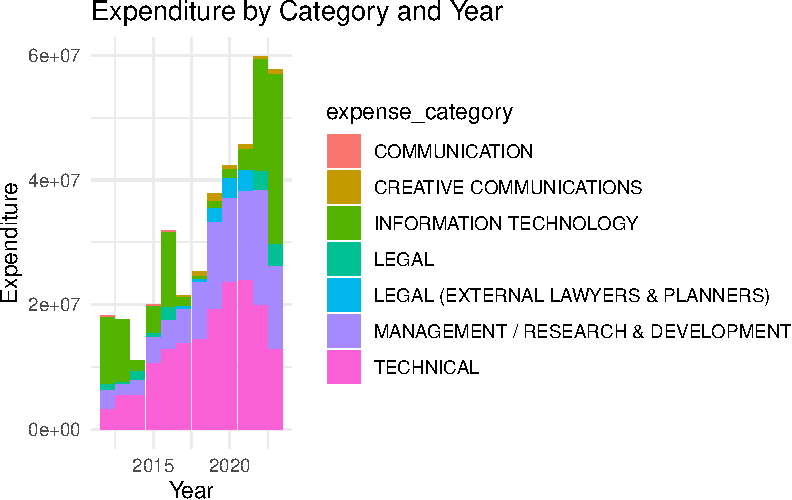
\includegraphics{paper_files/figure-pdf/yearly-cat-expenditure-1.pdf}

}

\caption{Yearly Expenditure by Category}

\end{figure}%

\begin{figure}[H]

{\centering 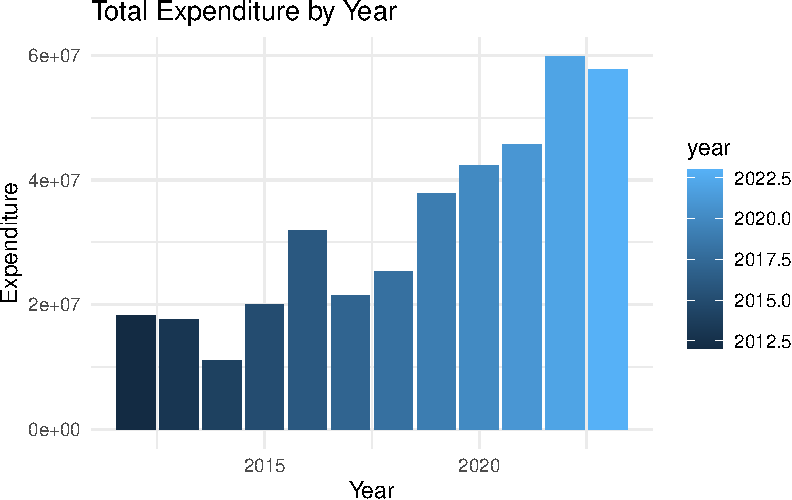
\includegraphics{paper_files/figure-pdf/top-consultants-1.pdf}

}

\caption{Expenditure by Consultant}

\end{figure}%

\begin{figure}[H]

{\centering 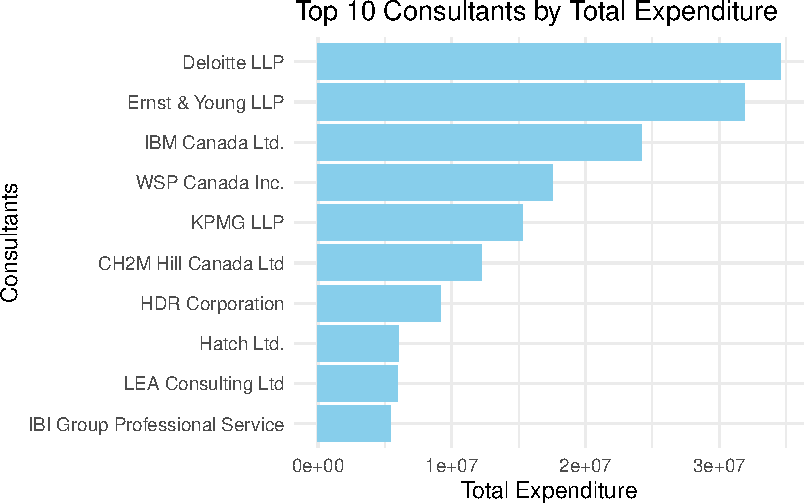
\includegraphics{paper_files/figure-pdf/top-consultants-2.pdf}

}

\caption{Expenditure by Consultant}

\end{figure}%

\begin{verbatim}
`summarise()` has grouped output by 'year'. You can override using the
`.groups` argument.
\end{verbatim}

\begin{verbatim}
Warning: Using `size` aesthetic for lines was deprecated in ggplot2 3.4.0.
i Please use `linewidth` instead.
\end{verbatim}

\begin{figure}[H]

{\centering 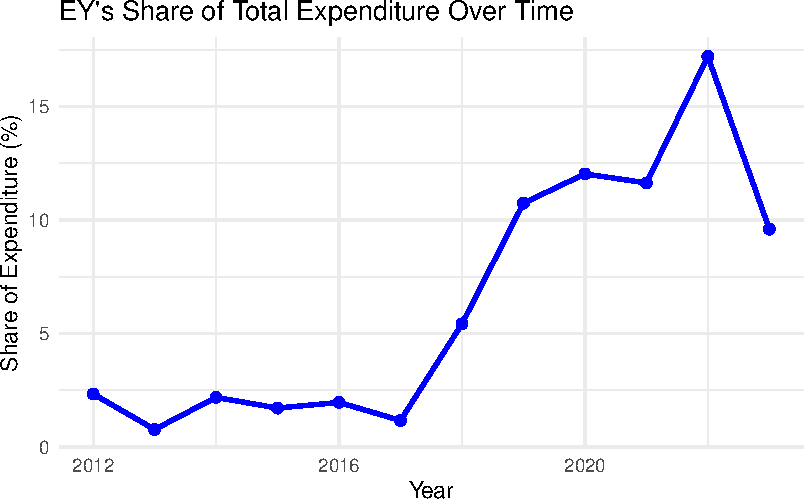
\includegraphics{paper_files/figure-pdf/increasing-share-proof-1.pdf}

}

\caption{Increasing Share of Total Expenditure}

\end{figure}%

\begin{figure}[H]

{\centering 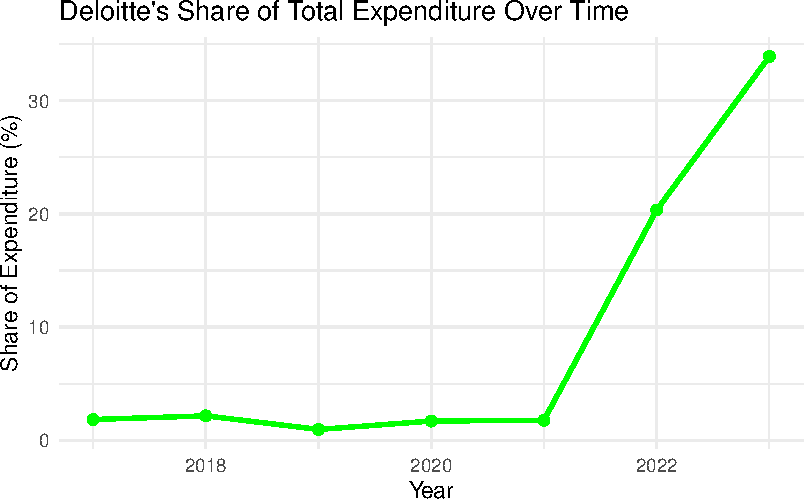
\includegraphics{paper_files/figure-pdf/increasing-share-proof-2.pdf}

}

\caption{Increasing Share of Total Expenditure}

\end{figure}%

\section{Discussion\{sec-discussion\}}\label{discussionsec-discussion}

\subsection{Weaknesses and next
steps\{sec-future-work\}}\label{weaknesses-and-next-stepssec-future-work}

Weaknesses and next steps should also be included.

\newpage

\appendix

\section*{Appendix}\label{appendix}
\addcontentsline{toc}{section}{Appendix}

\section{Additional data details}\label{additional-data-details}

\newpage

\section*{References}\label{references}
\addcontentsline{toc}{section}{References}

\phantomsection\label{refs}
\begin{CSLReferences}{1}{0}
\bibitem[\citeproctext]{ref-ArriveCANScandalFacts}
Canada. 2024. {``Procurement Practice Review of ArriveCAN - Office of
the Procurement Ombudsman.''} \emph{Opo-Boa.gc.ca}.
\url{https://opo-boa.gc.ca/praapp-prorev/2024/epa-ppr-01-2024-eng.html}.

\bibitem[\citeproctext]{ref-opendatatoronto}
Gelfand, Sharla. 2022. \emph{Opendatatoronto: Access the City of Toronto
Open Data Portal}.
\url{https://sharlagelfand.github.io/opendatatoronto/}.

\bibitem[\citeproctext]{ref-citeR}
R Core Team. 2023. \emph{R: A Language and Environment for Statistical
Computing}. Vienna, Austria: R Foundation for Statistical Computing.
\url{https://www.R-project.org/}.

\bibitem[\citeproctext]{ref-ggplot2}
Wickham, Hadley. 2016. \emph{Ggplot2: Elegant Graphics for Data
Analysis}. Springer-Verlag New York.
\url{https://ggplot2.tidyverse.org}.

\bibitem[\citeproctext]{ref-tidyverse}
Wickham, Hadley, Mara Averick, Jennifer Bryan, Winston Chang, Lucy
D'Agostino McGowan, Romain François, Garrett Grolemund, et al. 2019.
{``Welcome to the {tidyverse}.''} \emph{Journal of Open Source Software}
4 (43): 1686. \url{https://doi.org/10.21105/joss.01686}.

\end{CSLReferences}




\end{document}
